\documentclass[a4paper,twoside]{article}

\usepackage{balance}
\usepackage{epsfig}
\usepackage{subcaption}
\usepackage{calc}
\usepackage{amsfonts}
\usepackage{amssymb}
\usepackage{amstext}
\usepackage{amsmath}
\usepackage{amsthm}
\usepackage{array}
\usepackage{booktabs}
\usepackage{cite}
\usepackage{enumitem}
\usepackage{graphicx}
\usepackage{hyperref}
\usepackage{multicol}
\usepackage{pslatex}
\usepackage{algorithm2e}
\usepackage{xcolor}
\usepackage{interval}
\usepackage[font=scriptsize]{caption}
\usepackage[bottom]{footmisc}

\usepackage{SCITEPRESS}


\graphicspath{ {./img/} }
\intervalconfig{
    soft open fences,
}

\begin{document}
\title{Appendix}
\section{PyResolveMetrics Technology}\label{appendix:technology}
    The proposed library is implemented using the Python programming
    language (version 3.11)\cite{python}.
    It makes use of the Numpy library\cite{harris2020numpy} to accelerate
    the expensive computations required by some of the implemented metrics.
    The library does not pose any additional hardware or software portability
    issues over the ones that are specific to Python and Numpy.
    In fact, the library design values portability and a high level of
    interoperability above other desirable traits such as performance and does
    so first and foremost by abiding to existing standards.

    Python propagates standards throughout the community using protocols.
    Python protocols\cite{pyproto2017} provide a clean and effortless way to
    integrate new components, libraries and applications within the Python
    ecosystem.
    While other libraries\cite{nmeth2020scipy} promote their own API by
    requiring users to adapt their data to the strictures of the library design,
    our library takes full advantage of the Python ecosystem by leveraging
    protocols, such as \texttt{Iterable} and \texttt{Hashable}.

    All our library functions expect \texttt{Iterable} sequences as their input.
    In fact, the ground truth and ER result can be any
    \texttt{Iterable} data structure that complies with the ER
    model of choice.
    For the statistical model, the library accepts \texttt{Iterable[tuple]}
    input arguments, where the inner tuple must contain only two items.
    For the algebraic model, the library represents partitions as
    \texttt{Iterable[set]} instances.
    Since sets operate on \texttt{Hashable} items, any instance that implements
    the \texttt{Hashable} protocol is compatible with the library.
    
    Adhering to the \texttt{Hashable} protocol has some less obvious advantages
    over imposing design choices onto the user to compute metrics:
    \begin{itemize}
        \item it works out of the box with basic types such as numbers or
        strings, but also with any \texttt{Hashable} types such as tuples or
        lists;
        \item if custom objects are used to represent the data that describes
        entities, the objects can be reused when computing metrics thus saving
        the memory that would otherwise be allocated for labeling the data;
        \item the only adaptation required to use this library is implementing
        the well-known \texttt{Hashable} protocol, leading to a much lower
        implementation effort in the case when the data is not already
        compatible with the library\@
    \end{itemize}

    Choosing Python deserves special attention also because of a limitation it
    imposes on the design.
    Normally, a partition $P$ over a set $X$ is defined as a set of
    non-overlapping subsets containing all the elements from $X$, that is:
    \begin{equation}
        P(X) = \{ C_1, C_2, \ldots, C_n | \bigcap\limits^n_{i=1}C_i=\emptyset \land \bigcup\limits^n_{i=1}C_i=X \}
    \end{equation}
    The library implements metrics that compare partitions, but it requires the
    partition to be specified as an \texttt{Iterable[set]} instead of a set of
    sets.

    The reason behind this choice is purely technological and lies with the
    choice of the Python core team to not make \texttt{set} instances
    \texttt{Hashable}.
    This entails an obligation on the part of the library to verify that, when
    partitions over a set are expected as the input arguments of a library
    function, that function will verify that the input arguments are partitions
    over the same set.

    Using the \texttt{frozenset} data type (which is \texttt{Hashable}) instead
    of the \texttt{Iterable} protocol would decrease the interoperability of the
    library.
    The gains of choosing the \texttt{frozenset} in terms of performance and
    maintainability of the library would be marginal because checking that two
    iterable sequences of sets are partitions over the same set is a trivial and
    efficient algorithm that needs to be implemented only once.

    While the library does focus on interoperability and portability, it does
    not disregard performance.
    The most notable design choice that increases the computational and memory
    efficiency of the library has to do with adopting Numpy as a primary
    dependency.
    Numpy helps by externalizing resource intensive calculations (especially
    those that are required for clustering metrics) to subroutines that are
    compiled to native machine code.

    \section{Example Usage: Plots for Metrics}\label{appendix:sample-figures}
    This section contains the plots of the metrics computed after running the
    PPJoin algorithm on DG1 and DG2 for values of $t$ in the interval
    $\rinterval{0}{1}$ at increments of $0.01$.

    The plots for the probabilistic metrics are available in
    Figure~\ref{appendix:fig:fs-figures}.

    \begin{figure*}[htbp]
        \begin{minipage}{0.32\textwidth}
            \centering
            \caption*{Precision}
            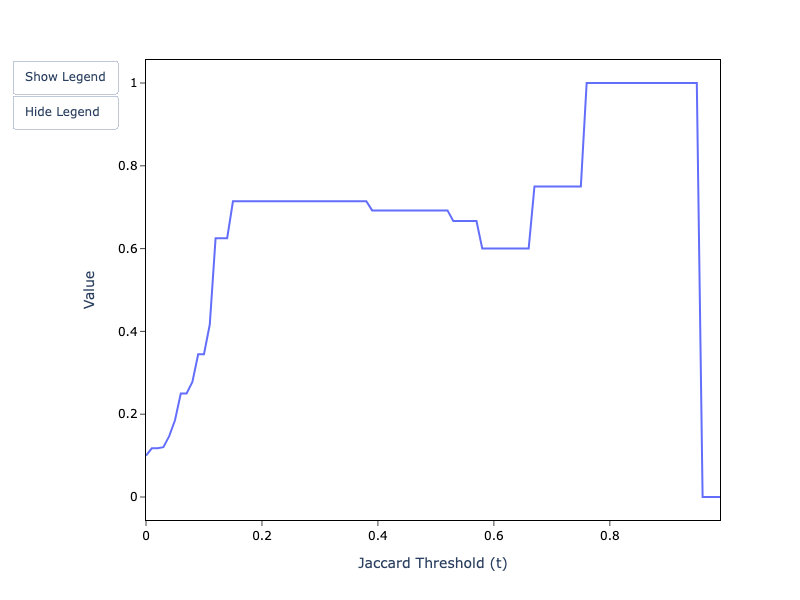
\includegraphics[width=\textwidth]{sample-usage/mini-fs-precision}
        \end{minipage}    
        \begin{minipage}{0.32\textwidth}
            \centering
            \caption*{Recall}
            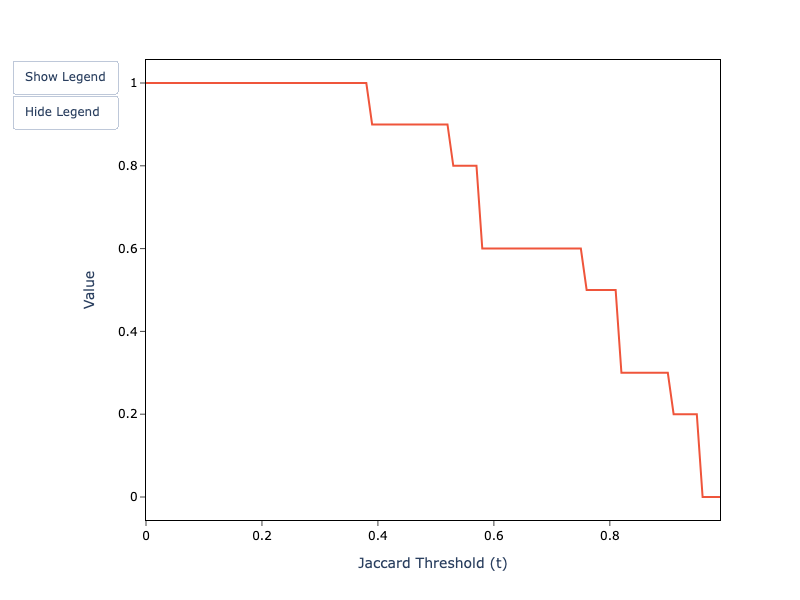
\includegraphics[width=\textwidth]{sample-usage/mini-fs-recall}
        \end{minipage}    
        \begin{minipage}{0.32\textwidth}
            \centering
            \caption*{$F_1$}
            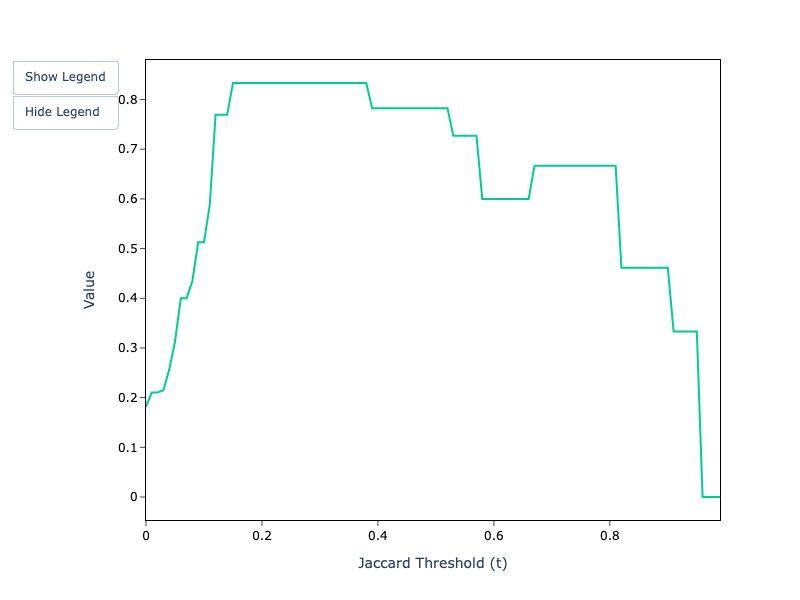
\includegraphics[width=\textwidth]{sample-usage/mini-fs-f1}
        \end{minipage}
        \caption{Fellegi-Sunter Metrics}\label{appendix:fig:fs-figures}
    \end{figure*}

    Pairwise metrics are depicted in Figure~\ref{appendix:fig:alg-pairwise}.

    \begin{figure*}[htbp]
        \begin{minipage}{0.32\textwidth}
            \centering
            \caption*{Pairwise Precision}
            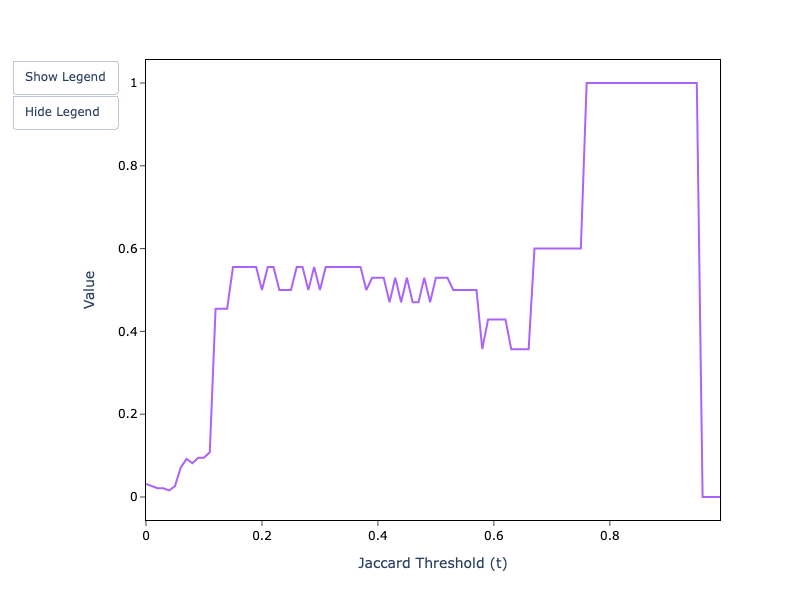
\includegraphics[width=\textwidth]{sample-usage/mini-alg-pp}
        \end{minipage}    
        \begin{minipage}{0.32\textwidth}
            \centering
            \caption*{Pairwise Recall}
            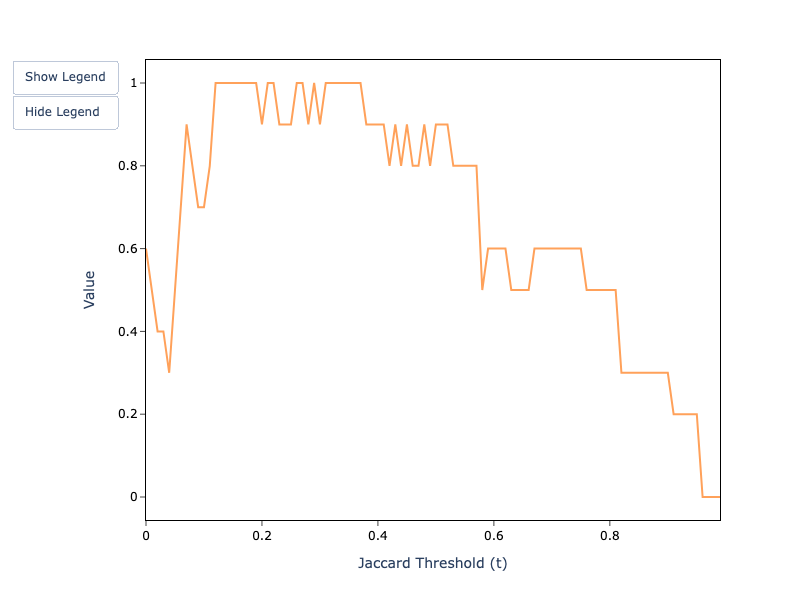
\includegraphics[width=\textwidth]{sample-usage/mini-alg-pr}
        \end{minipage}    
        \begin{minipage}{0.32\textwidth}
            \centering
            \caption*{Pairwise F Measure}
            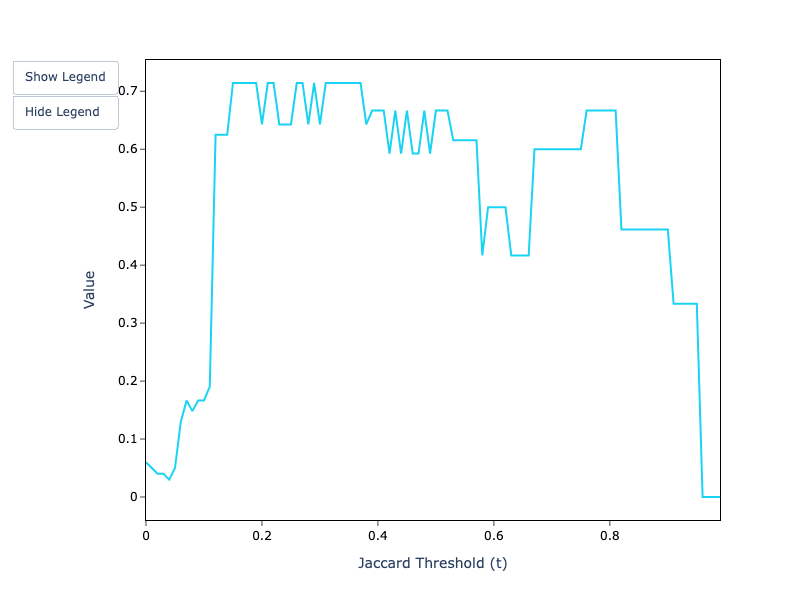
\includegraphics[width=\textwidth]{sample-usage/mini-alg-pf}
        \end{minipage}
        \caption{Pairwise Metrics}\label{appendix:fig:alg-pairwise}
    \end{figure*}

    Cluster metrics can be viewed in  Figure~\ref{appendix:fig:alg-cluster}.

    \begin{figure*}[htbp]
        \begin{minipage}{0.32\textwidth}
            \centering
            \caption*{Cluster Precision}
            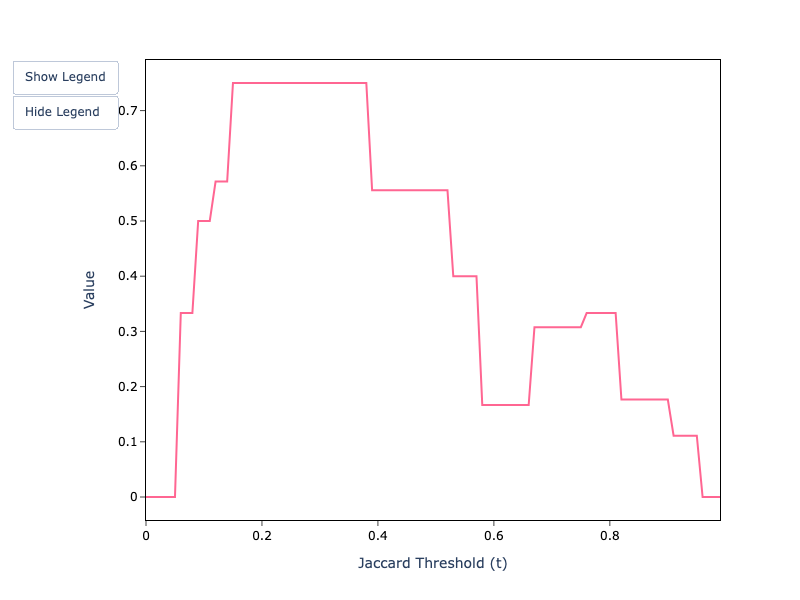
\includegraphics[width=\textwidth]{sample-usage/mini-alg-cp}
        \end{minipage}    
        \begin{minipage}{0.32\textwidth}
            \centering
            \caption*{Cluster Recall}
            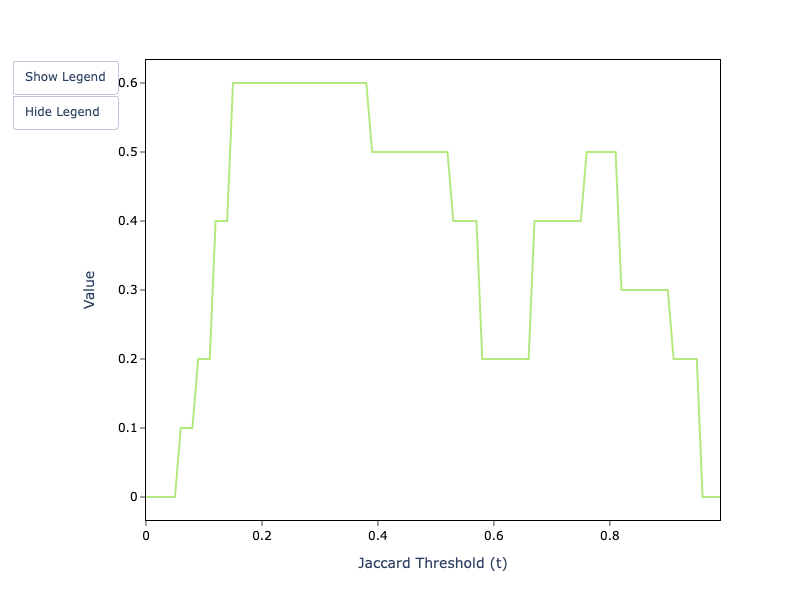
\includegraphics[width=\textwidth]{sample-usage/mini-alg-cr}
        \end{minipage}    
        \begin{minipage}{0.32\textwidth}
            \centering
            \caption*{Cluster F Measure}
            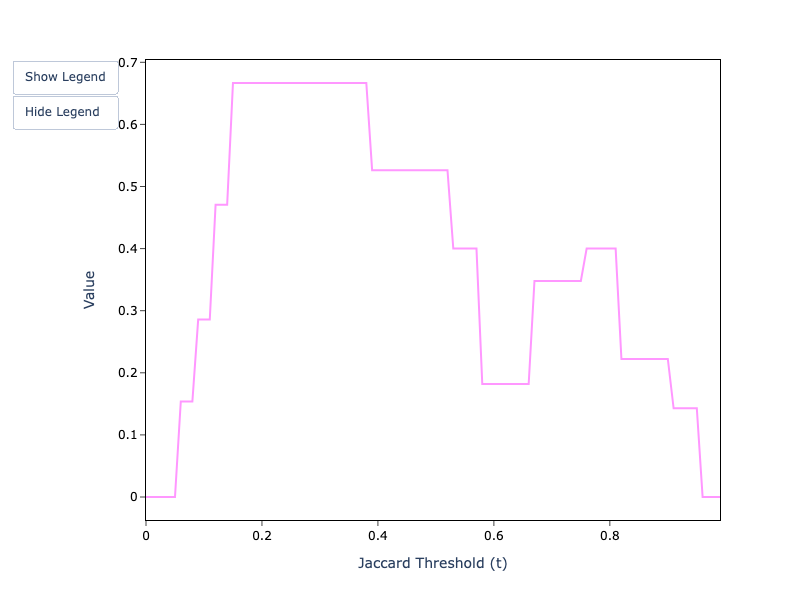
\includegraphics[width=\textwidth]{sample-usage/mini-alg-cf}
        \end{minipage}
        \caption{Cluster Metrics}\label{appendix:fig:alg-cluster}
    \end{figure*}

    We showcase the algebraic indexes in Figure~\ref{appendix:fig:alg-indexes}.

    \begin{figure*}[htbp]
        \begin{minipage}{0.32\textwidth}
            \centering
            \caption*{Talburt-Wang Index}
            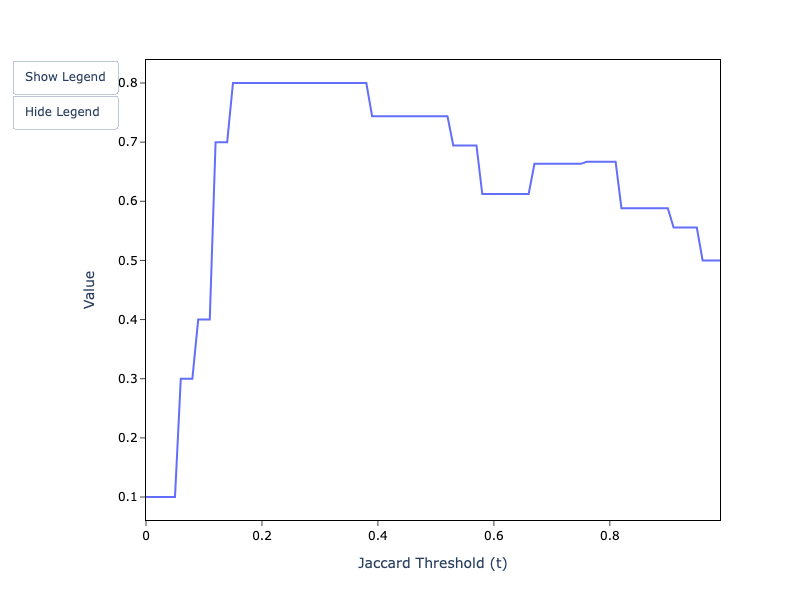
\includegraphics[width=\textwidth]{sample-usage/mini-alg-twi}
        \end{minipage}    
        \begin{minipage}{0.32\textwidth}
            \centering
            \caption*{Rand Index}
            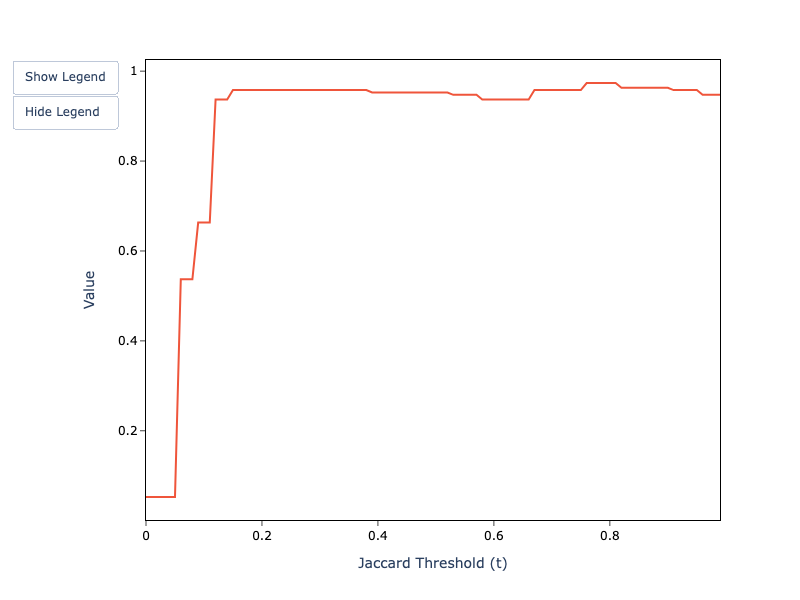
\includegraphics[width=\textwidth]{sample-usage/mini-alg-ri}
        \end{minipage}    
        \begin{minipage}{0.32\textwidth}
            \centering
            \caption*{Adjusted Rand Index}
            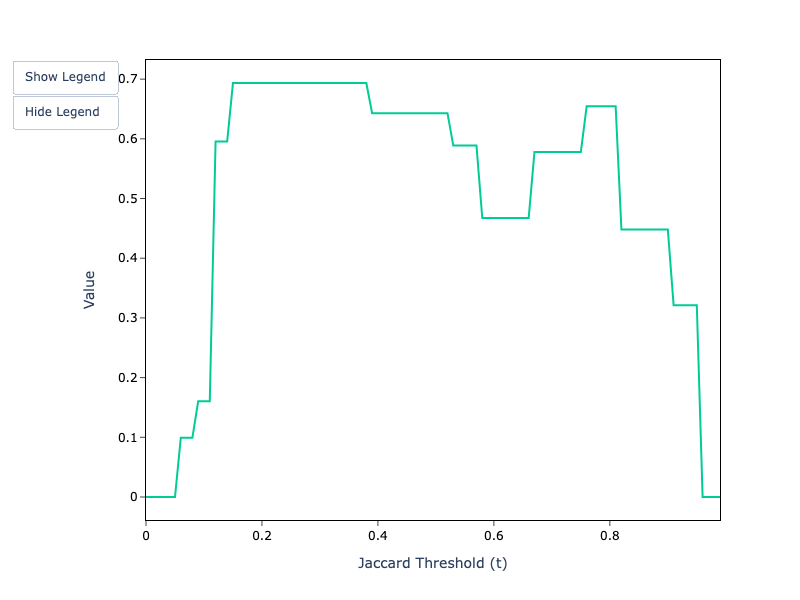
\includegraphics[width=\textwidth]{sample-usage/mini-alg-ari}
        \end{minipage}
        \caption{Algebraic Model Indexes}\label{appendix:fig:alg-indexes}
    \end{figure*}

    \section{Performance Evaluation Data}\label{appendix:sec:perf}
    This section contains figures and tables concerning the performance of the
    PyResolveMetrics library.

    We use flamegraphs\cite{flamegraphs2013} to represent the CPU usage
    patterns in the library and the \texttt{cProfile} package from the Python
    standard library to trace the execution of the functions that compute
    metrics.
    The flame graph from Figure~\ref{appendix:fig:fs-cpu-perf}
    shows that the Fellegi-Sunter metrics take up less CPU than the validation
    of the input and output of data. 
    The main consumers are shown in Table~\ref{appendix:table:fs-cpu-perf}.  
    The best lesson we can learn here is that computing the statistical metrics
    is not resource-intensive at all. 

    The same cannot be said about the metrics that work with partitions over an
    input set. 
    Table~\ref{appendix:table:alg-cpu-perf} presents how the algebraic metrics perform. 
    The pairwise and cluster metrics still perform well as indicated in
    Figure~\ref{appendix:fig:alg-cpu-perf}. 
    However, when we move on to consider the performance of the three supported
    indices, we see that computing the Rand Index and the Adjusted Rand Index
    prove to be the most onerous operations by far. 
    We take note that the \texttt{\char`_convert\char`_to\char`_algebraic}
    function that checks whether the metrics are applied to two partitions over
    the same set is also a large consumer of CPU time.
    However, since that function is executed nine times (once for computing each
    metric) we declare ourselves content to file a note to improve the
    performance of that function at a later time.

    \begin{figure*}[htbp]
        \centering
        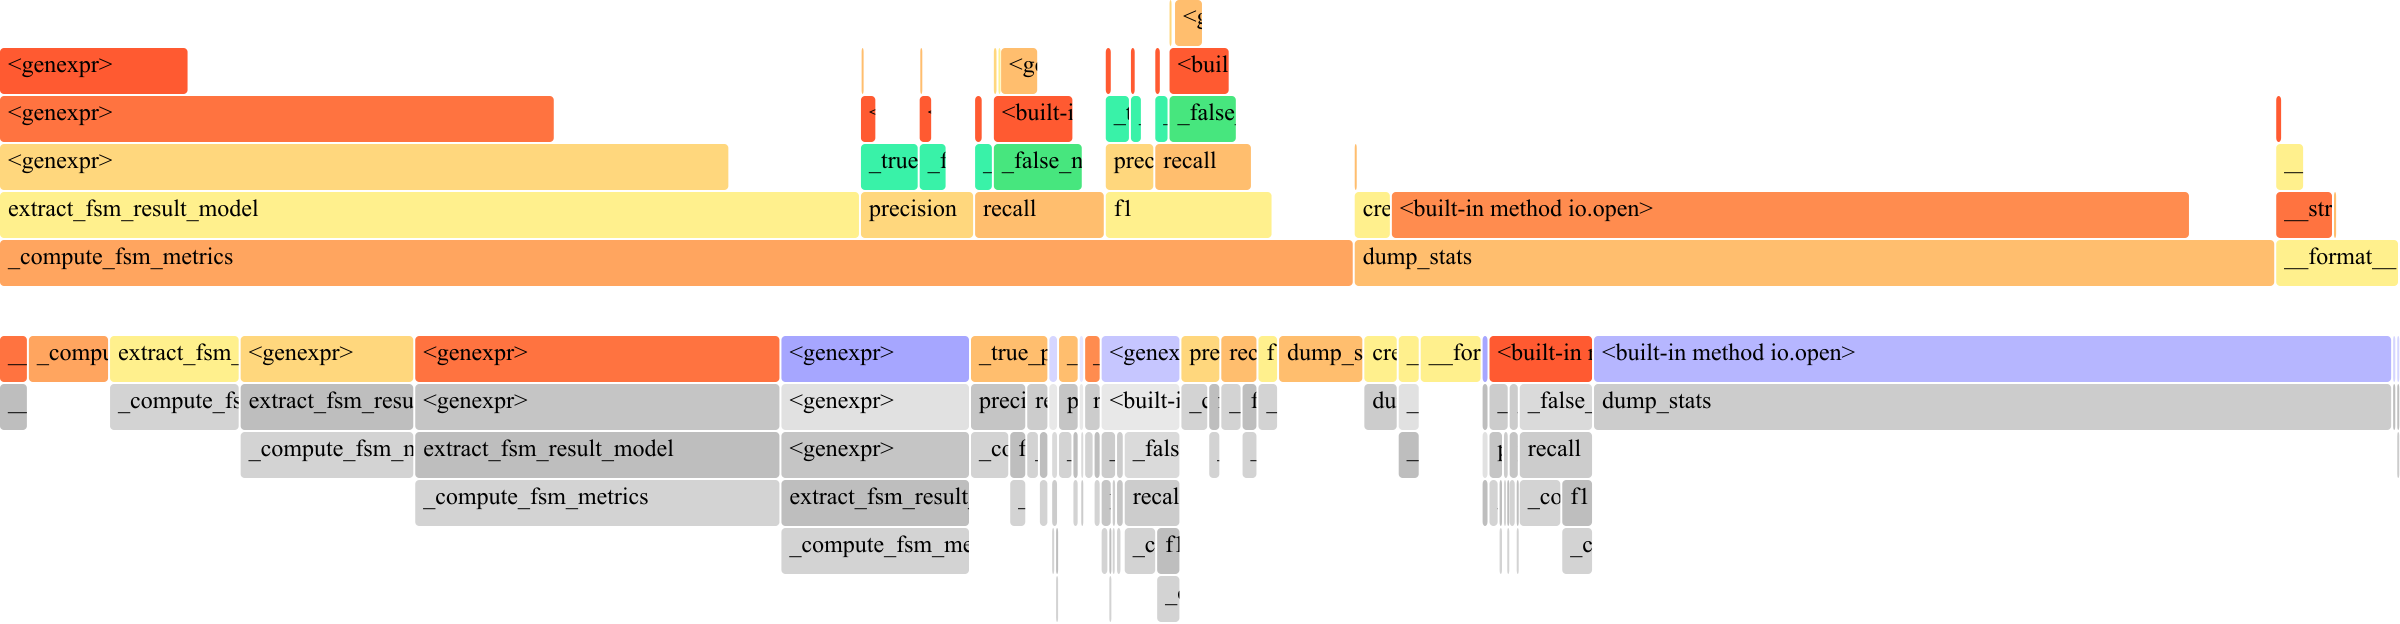
\includegraphics[width=\textwidth]{performance/fs-flamegraph}
        \caption{Fellegi-Sunter CPU Performance}\label{appendix:fig:fs-cpu-perf}
    \end{figure*}

    \begin{table*}[htbp]
        \centering
        \begin{tabular}{c c c c}
            \toprule
            Metric & Cumulative Time & Number of Calls & Time per Call \\ [0.5ex]
            \toprule
            \texttt{recall} & 7.208e-06 & 2 & 3.604e-06 \\
            \midrule
            \texttt{f1} & 5.291e-06 & 1 & 5.291e-06 \\
            \midrule
            \texttt{precision} & 4.75e-06 & 2 & 2.375e-06 \\
            \bottomrule
        \end{tabular}
        \caption{Fellegi-Sunter Metrics}\label{appendix:table:fs-cpu-perf}
    \end{table*}

    \begin{figure*}[htbp]
        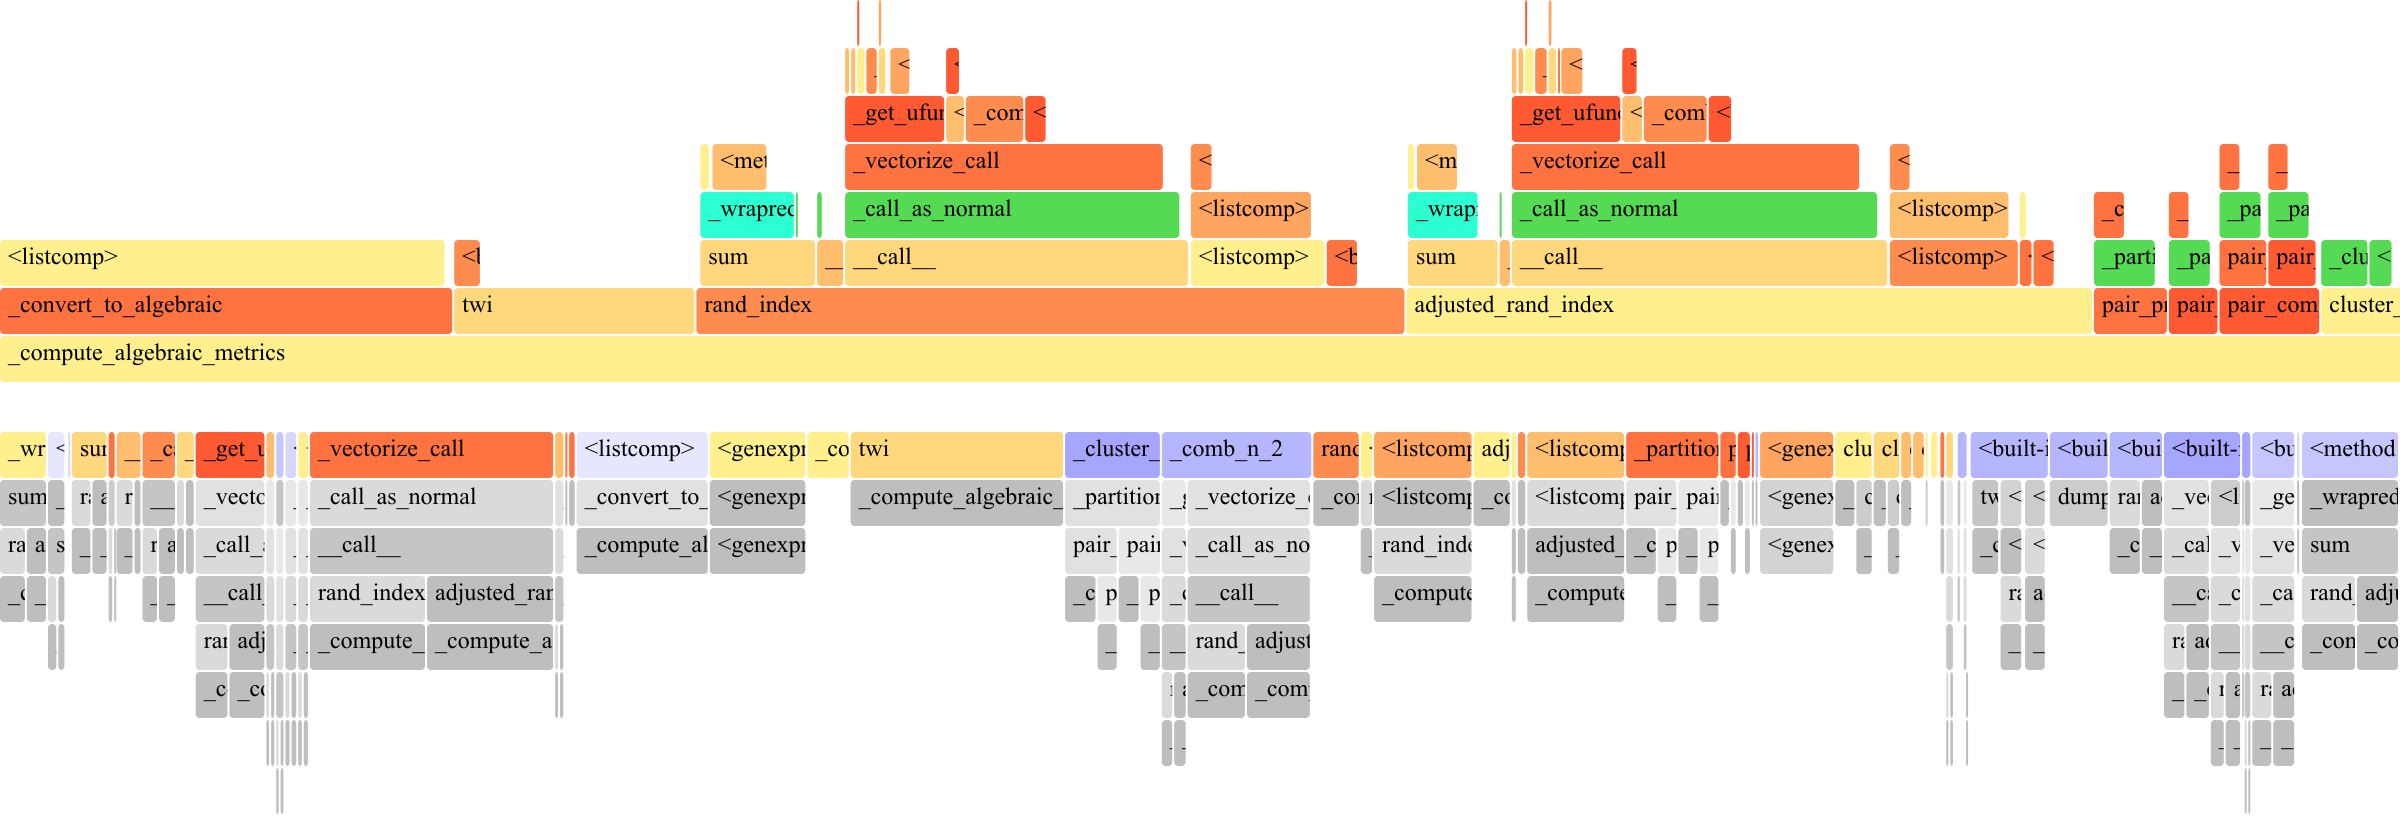
\includegraphics[width=\textwidth]{performance/algebraic-flamegraph}
        \caption{Algebraic CPU Performance}\label{appendix:fig:alg-cpu-perf}
    \end{figure*}

    \begin{table*}[ht!]
        \centering
        \begin{tabular}{c c c c}
            \toprule
            Metric & Cumulative Time & Number of Calls & Time per Call \\ [0.5ex]
            \toprule
            \texttt{rand\char`_index} & 0.0004027 & 1 & 0.0004027 \\
            \midrule
            \texttt{adjusted\char`_rand\char`_index} & 0.0001944 & 1 & 0.0001944 \\
            \midrule
            \texttt{twi} & 9.146e-05 & 1 & 9.146e-05 \\
            \midrule
            \texttt{cluster\char`_comparison\char`_measure} & 5.35e-05 & 1 & 5.35e-05 \\
            \midrule
            \texttt{cluster\char`_recall} & 5.154e-05 & 2 & 2.577e-05 \\
            \midrule
            \texttt{cluster\char`_precision} & 4.271e-05 & 2 & 2.135e-05 \\
            \midrule
            \texttt{pair\char`_precision} & 2.971e-05 & 2 & 1.485e-05 \\
            \midrule
            \texttt{pair\char`_recall} & 2.613e-05 & 2 & 1.306e-05 \\
            \midrule
            \texttt{pair\char`_comparison\char`_measure} & 2.596e-05 & 1 & 2.596e-05 \\
            \bottomrule
        \end{tabular}
        \caption{Algebraic Metrics}\label{appendix:table:alg-cpu-perf}
    \end{table*}


\bibliographystyle{apalike}
{
    \small
    \bibliography{03_references}
}
\end{document}